\subsection{Personas von NUNAV-Nutzern}
\label{sec:06_model_evaluation:personas}

Um die Interpretation der Rohanforderungen aus dem durchgeführten Workshop besser interpretieren zu können, wurden Personas für typische NUNAV-Nutzergruppen abgeleitet. \textit{Graphmasters} hat zwar kein genaues Bild, darüber welche Nutzertypen \textit{NUNAV Navigation} nutzen, aus vergangenen Nutzergesprächen und Feedback haben sich allerdings zwei Gruppen herauskristallisiert, die klar benennbar sind.

\begin{wrapfigure}{o}{0.33\textwidth}
    \vspace{-\intextsep}
    \centering
    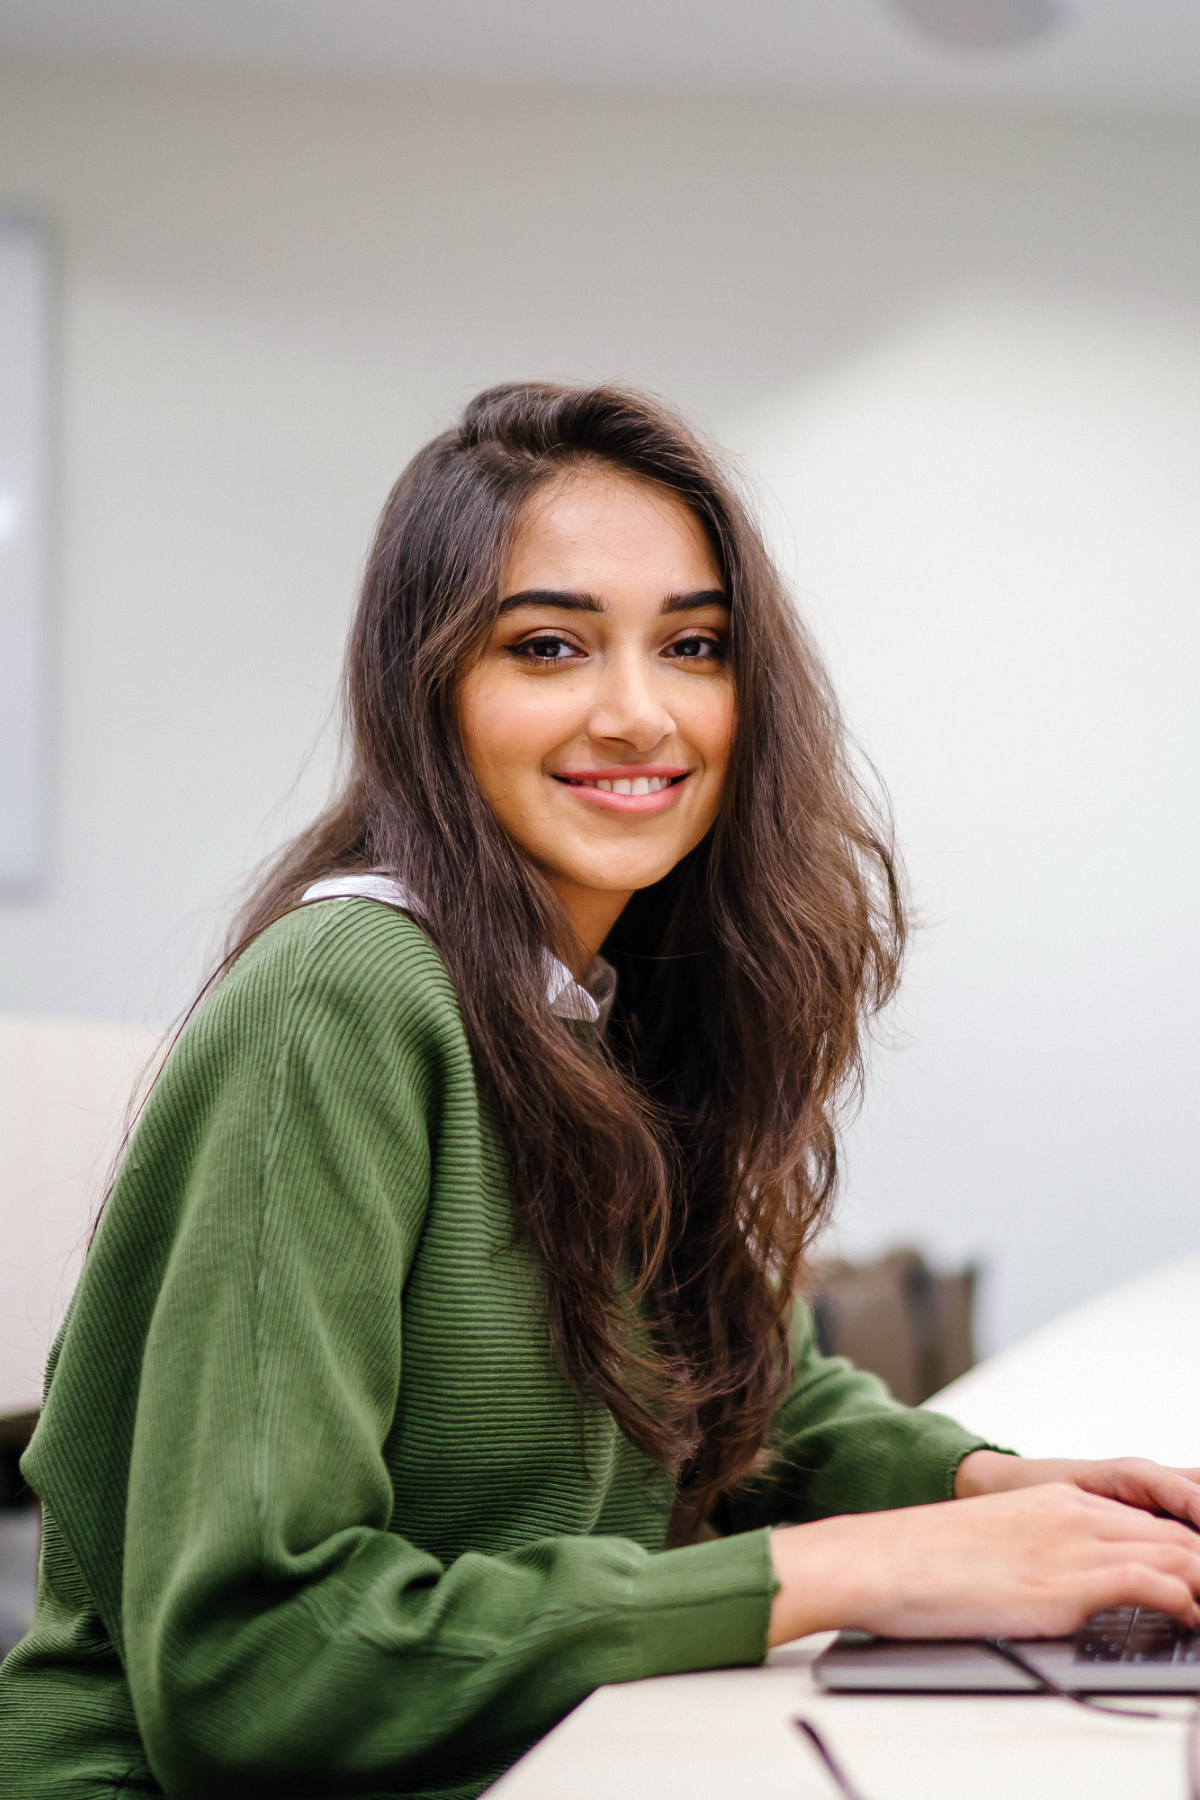
\includegraphics[width=\textwidth]{contents/06_model_evaluation/01_integration/res/persona_picture_ayla.png}
    \caption[]{Ayla -\\Lizensiert bei Shutterstock Nr. 1433736386}
\end{wrapfigure}

\paragraph{Erstnutzerin:} Ayla ist 23 Jahre alt und studiert aktuell Mathematik im 7. Bachelorsemester. Sie wohnt in einem Studentenwohnheim und fährt jeden Tag mit der Bahn zur Universität. Sie kommt ursprünglich aus einem Dorf ca. 300~km entfernt und besucht ihre Eltern dort mindestens an drei Wochenenden im Monat. Dafür hat sie ein Auto, da sie mit ihrem Semesterticket nicht bis in die Heimat fahren kann. Sie wählt ihre Fahrtzeiten so, dass möglichst wenig Verkehr auf den Straßen ist.

In der Universität benutzt Ayla für Mitschriften und Notizen Zettel und Stift. Die Vorlesungsskripte druckt sie im Regelfall aus, um darin Notizen zu machen. Ihren Laptop nutzt sie nur, um die bereitgestellten Materialien der Dozenten herunterzuladen und mit ihnen zu kommunizieren. Folglich erledigt Ayla viele Aufgaben noch gerne analog statt digital. 

Sie ist sehr aktiv auf Social-Media-Kanälen und postet regelmäßig Bilder mit ihrem Smartphone der neusten Generation.

Ayla ist großer Fan von Rap-Musik. Einer ihrer Lieblings-Rapper gibt in Kürze ein einzelnes Konzert in Deutschland und sie konnte zusammen mit zwei Freundinnen an Karten kommen. Da sie ein Auto hat, wollen die drei zusammen mit dem Auto zum Konzert fahren. Vom Veranstalter haben sie eine E-Mail erhalten, dass zur Anreise mit dem Auto möglichst die App \textit{NUNAV Navigation} genutzt werden soll. Dies wollen sie ausprobieren.

\newpage

\begin{wrapfigure}{o}{0.33\textwidth}
    \vspace{-\intextsep}
    \centering
    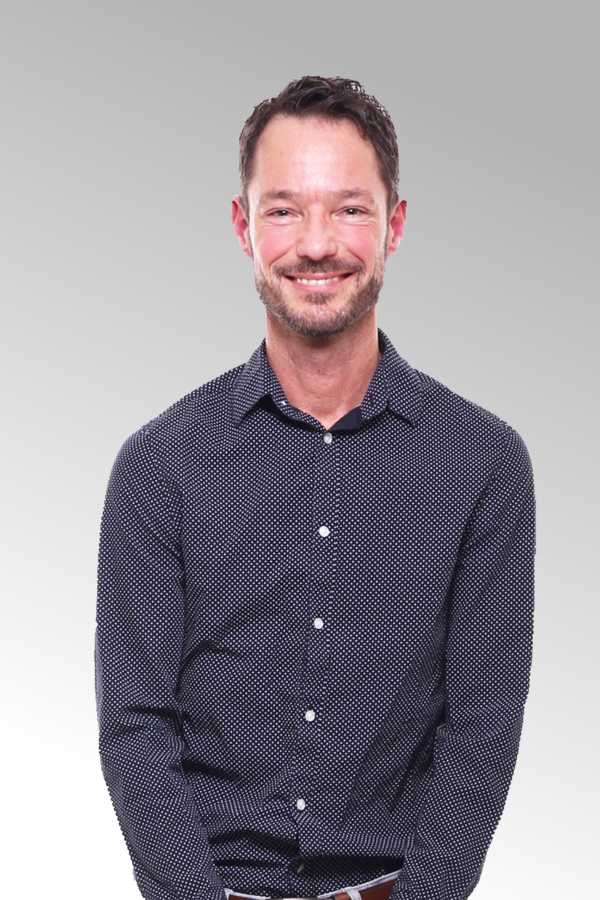
\includegraphics[width=\textwidth]{contents/06_model_evaluation/01_integration/res/persona_picture_michael.png}
    \caption[]{Michael -\\Lizensiert bei Shutterstock Nr. 602783837}
\end{wrapfigure}

\paragraph{Vielfahrer:} Michael, 34 Jahre alt, arbeitet als Unternehmensberater in einem großen Beratungsunternehmen. Er hat Betriebswirtschaftleere studiert und ist seit dem Studium in der Firma.

Er wohnt mit seiner Frau und einer Tochter in der Vorstadt und muss jeden Morgen zur Hauptverkehrsszeit in die Stadt fahren, um in sein Büro zu kommen. Dadurch steht er nahezu täglich auf dem Weg zur Arbeit im Stau. Die öffentlichen Verkehrsmittel kommen für ihn nicht in Frage, da er mit ihnen mehr als doppelt so lange bräuchte.

Auch zu Vorortterminen beim Kunden fährt er ungefähr einmal pro Woche. Dabei interessiert ihn vor allem, wie lange er für die Strecke benötigt und, dass er pünktlich ankommt.

Lange Zeit hat er das in sein Auto integrierte Navigationssystem verwendet, das aber nur vereinzelt auf Staus reagiert hat und ihn jeden Tag auf der gleichen Strecke zur Arbeit geschickt hat, wenn nicht ein besonderes Ereignis wie Unfälle oder Sperrungen auf der Strecke waren.

Michael hat ein modernes Dienst-Smartphone mit Android und ist generell Technik interessiert. Zwischendurch hat er die auf seinem Smartphone vorinstallierte Navigations-App verwendet, da diese den aktuellen Verkehr anzeigen kann. Diese leitete ihn zum Teil aus dem Stau des Berufsverkehrs raus, in dem er stand. Er hat aber meist ähnlich lange zur Arbeit gebraucht wie im Stau. Außerdem achtet Michael darauf, was mit seinen Daten passiert und da ist er sich bei dem Anbieter unsicher, wie anonym diese verarbeitet werden.

Seit einigen Tagen verwendet er die Navigations-App \text{NUNAV Navigation}, die verspricht ihn jeden Tag auf dem schnellsten Weg zur Arbeit zu bringen. Die App schlägt ihm ab und zu seiner Meinung nach \glqq komische\grqq{} Routen vor. Anfangs hat er sich dann nicht an diese gehalten. Später hat er die NUNAV-Routen vollständig ausprobiert und war tatsächlich etwas schneller als sonst auf dem Weg zur Arbeit. Michael ist aber immer noch skeptisch, da er die vorgeschlagenen Routen nicht immer versteht und sich bei Umwegen daher immer noch auf seine Intuition verlässt.

\newpage